\documentclass[12pt,letter]{article}
\usepackage{geometry}\geometry{top=0.75in}
\usepackage{amsmath}
\usepackage{amssymb}
\usepackage{mathtools}
\usepackage{xcolor}	% Color words
\usepackage{cancel}	% Crossing parts of equations out
\usepackage{tikz}    	% Drawing 
\usepackage{pgfplots}   % Other plotting
\usepgfplotslibrary{colormaps,fillbetween}
\usepackage{placeins}   % Float barrier
\usepackage{hyperref}   % Links
\usepackage{tikz-qtree} % Trees
\usepackage{graphicx}
\usepackage{subcaption}

%\tikzset{
%    treenode/.style = {shape=rectangle, rounded corners, draw, align=center}
%    root/.style     = {treenode, font=\Large}
%    env/.style      = {treenode, font=\ttyfamily\normalsize},
%    dummy/.style    = {circle,draw}
%}

%\tikzset{every tree node/.style={circle,align=center, anchor=west, grow=right}
%	}
\tikzset{every tree node/.style={align=center,minimum width=2em},%, draw},%, circle},
	 grow=right,
	 level distance=1.75cm}

% Don't indent
\setlength{\parindent}{0pt}
% Function to replace \section with a problem name specifically formatted
\newcommand{\problem}[1]{\vspace{3mm}\Large\textbf{{Problem {#1}\vspace{3mm}}}\normalsize\\}
% Formatting function, like \problem
\newcommand{\ppart}[1]{\vspace{2mm}\large\textbf{\\Part {#1})\vspace{2mm}}\normalsize\\}
% Formatting 
\newcommand{\condition}[1]{\vspace{1mm}\textbf{{#1}:}\normalsize\\}

\begin{document}
\title{CIS 572 Assignment 1}
\author{Steven Walton}
\maketitle
\problem{1}
Answer Exercise 3.1 from 
\href{https://www.cs.princeton.edu/courses/archive/spr07/cos424/papers/mitchell-dectrees.pdf}{Chapter 3 of Mitchell's machine learning book.}

\ppart{a} 
$$ A \wedge\neg B$$
\begin{figure}[h]
\centering
\begin{tikzpicture}
%\Tree [.A [.T [.B [.T 0 ] [.F 1 ] ] ] [.F 0 ] ]
\Tree [.A [.T [.B [.T 0 ] [.F 1 ] ] ] [.F 0 ] ]
\end{tikzpicture}
\caption{$A\wedge\neg B$}
\end{figure}


\ppart{b}
$$A\vee (B\wedge C)$$
\begin{figure}[h]
\centering
\begin{tikzpicture}
\Tree [.A [.T 1 ] [.F [.B [.T [.C [.T 1 ] [.F 0 ] ] ] [.F 0 ] ] ] ]
\end{tikzpicture}
\caption{$A\vee(B\wedge C)$}
\end{figure}


\ppart{c}
$$ A\ \mathsf{XOR}\ B $$
\begin{figure}[h]
\centering
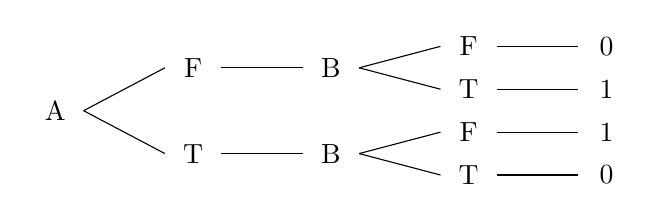
\begin{tikzpicture}
\Tree [.A [.T [.B [.T 0 ] [.F 1 ] ] ] [.F [.B [.T 1 ] [.F 0 ] ] ] ]
\end{tikzpicture}
\caption{$A\ \mathsf{XOR}\ B$}
\end{figure}

\ppart{d}
$$ (A\wedge B)\vee(C\wedge D)$$
\begin{figure}[h]
\centering
\begin{tikzpicture}
\Tree [.A [.T [.B [.T 1 ] [.F 0 ] ] ] [.F [.C [.T [.D [.T 1 ] [.F 0 ] ] ] [.F 0 ] ] ] ]
\end{tikzpicture}
\caption{$(A\wedge B)\vee(C\wedge D)$}
\end{figure}

\FloatBarrier
\problem{2}
Consider the samples in the Play-tennis dataset from Table $3.2$ in Mitchell's
textbook. If you calculate the information-gain for all of the attributes of this
set, you will observe that the attribute ``Outlook" has the largest information-
gain, which is equal to $0.246$. Therefore, the attribute ``Outlook" is the 
best heuristic choice for the root node.
\\
(a) List the labels of the new tree branches below the root node.
\\
(b) Which partition of the data will be assigned to each branch by ID3? Please
list the sample IDs that will be assigned to each branch.
\\
(c) Calculate the information gain for the remaining attributes in each branch, 
and determine which attribute will be chosen as the root of the sub-tree in
each branch.

\FloatBarrier
\ppart{a}
Now that we know that Overcast has the highest information gain, of $0.246$, we
will use it as the root node. We will then create the next nodes and show their
corresponding values for playing tennis or not, in the form of $\big[+yes,-no\big]$

\begin{figure}[h]
\centering
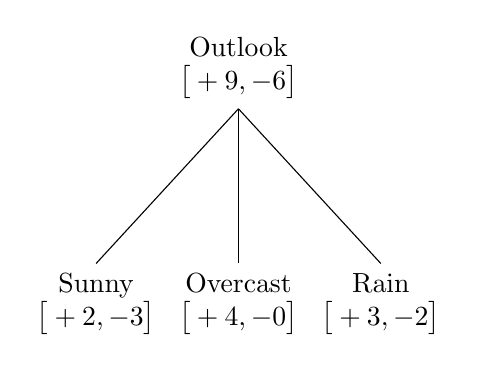
\begin{tikzpicture}[grow=down,level distance=3cm]
\Tree [.{Outlook\\$\big[+9,-6\big]$} [.{Sunny\\$\big[+2,-3\big]$} ] [.{Overcast\\$\big[+4,-0\big]$} ] [.{Rain\\$\big[+3,-2\big]$} ] ]
\end{tikzpicture}
\caption{Labels of new tree branches below root}
\end{figure}

\FloatBarrier
\ppart{b}
To determine how we will partition the data we will look at the entropy of each
node.

Given sunny, we have:

Humidity: High $\big[+0,-3\big]$, Normal $\big[+2,-0\big]$

Temperature: High $\big[+0,-2\big]$, Mild $\big[+1,-1\big]$, Cold $\big[+1,-0\big]$

Wind: Strong $\big[+1,-1\big]$, Weak $\big[+1,-2\big]$

\begin{align*}
S(Sunny,Humidity) &= S_{sunny} - S_{sunny,high} - S_{sunny,low}\\
	          &= S_{sunny} - \frac35(-1\log_2{1}) - \frac25(-1\log_2{1})\\
		  &= 0.97 - \frac35 0 - \frac25 0\\
		  &= 0.97
\end{align*}
We'll shorten steps from now on. We note that any $\big[+a,-a\big]=1$ and 
$\big[+a,0\big] = \big[0,-a\big] = 0$
\begin{align*}
S(Sunny,Temperature) &= S_{sunny} - S_{sunny,hot} - S_{sunny,mild} - S_{sunny,cold}\\
		     &= 0.97 - \frac250 - \frac251 - \frac250\\
		     &= 0.57
\end{align*}
\begin{align*}
S(Sunny,Wind) &= S_{sunny} - S_{sunny,strong} - S_{sunny,weak}\\
	      &= 0.97 - \frac251 - \frac35\left(-\frac13\log_2{\frac13} - \frac23\log_2{\frac23}\right)\\
	      &= 0.019
\end{align*}

From here we can see that the best thing to split on is humidity and the worst 
is wind. That gives us the following update to our tree.

\begin{figure}[h]
\centering
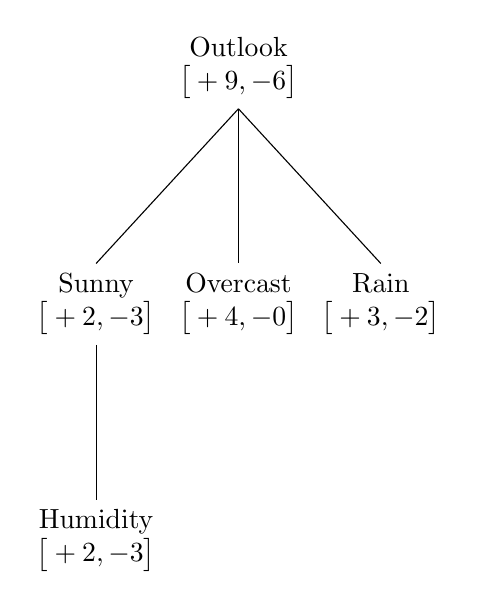
\begin{tikzpicture}[grow=down,level distance=3cm]
\Tree [.{Outlook\\$\big[+9,-6\big]$} [.{Sunny\\$\big[+2,-3\big]$} [.{Humidity\\$\big[+2,-3\big]$} ] ] [.{Overcast\\$\big[+4,-0\big]$} ] [.{Rain\\$\big[+3,-2\big]$} ] ]
\end{tikzpicture}
\caption{Partition of data}
\end{figure}

\FloatBarrier
\ppart{c}
Continuing with this process we get the following tree

\begin{figure}[h]
\centering
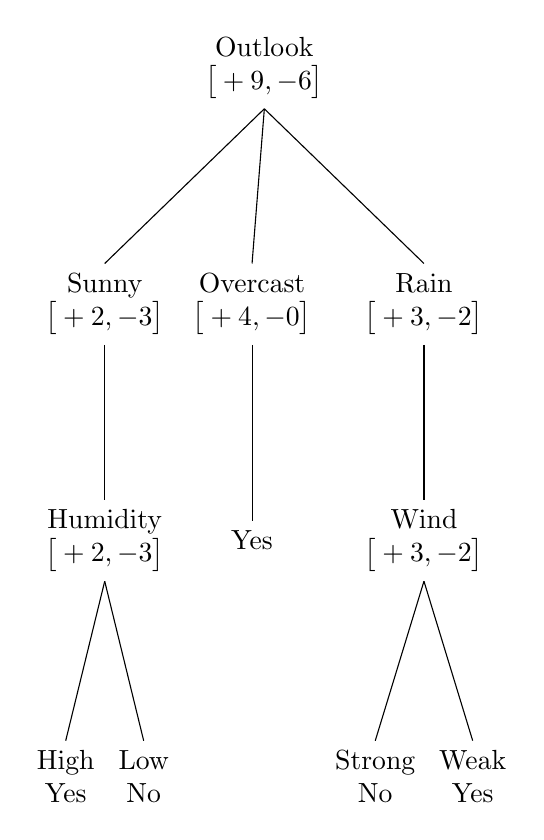
\begin{tikzpicture}[grow=down,level distance=3cm]
\Tree [.{Outlook\\$\big[+9,-6\big]$}
	[.{Sunny\\$\big[+2,-3\big]$}
	  [.{Humidity\\$\big[+2,-3\big]$} {High\\Yes} {Low\\No} ] 
        ]
	[.{Overcast\\$\big[+4,-0\big]$} Yes ]
	[.{Rain\\$\big[+3,-2\big]$}
	  [.{Wind\\$\big[+3,-2\big]$} {Strong\\No} {Weak\\Yes} ]
	]
      ]
\end{tikzpicture}
\caption{Full tree}
\end{figure}

\FloatBarrier
\problem{3}
Suppose a bank makes loan decisions using two decision trees, one that uses
attributes related to credit history and one that uses other demographic 
attributes. Each decision tree separately classifies a loan application as 
``High Risk" or ``Low Risk". The bank only offers a loan when both decision
trees predict ``Low Risk"

(a) Describe an algorithm for converting this pair of decision trees into a 
single decision tree that makes the same predictions (that is, it predicts
non-risky only when both of the original decision trees would have predicted 
non-risky).

(b) Let $n_1$ and $n_2$ be the number of leaves in the first and second decision
trees, respectively. Provide an upper bound on $n$, the number of leaves in the 
single equivalent decision tree, expressed as a function of $n_1$ and $n_2$.

\FloatBarrier
\ppart{1}
A simple method to combine the two trees is to just attach one of the trees to
all ``Low Risk" leaves of the other tree. We only need to check the ``Low Risk" 
leaves because a ``High Risk" leaf is already ruled out. A simplified example 
is shown below in Figure \ref{fig:example} and Figure \ref{fig:combined}.

\begin{figure}[h]
\centering
    \begin{subfigure}[b]{0.45\textwidth}
        \begin{tikzpicture}[grow=down,level distance=3cm]
             \hspace{2cm}\Tree [.{C1} [.C2 H L ] [.C3 H L ] ]
        \end{tikzpicture}
        \caption{Credit History}
    \end{subfigure}
    \begin{subfigure}[b]{0.45\textwidth}
        \begin{tikzpicture}[grow=down,level distance=3cm]
            \hspace{2cm}\Tree [.{D1} [.D2 H L ] [.D3 H L ] ]
        \end{tikzpicture}
	\caption{Demographic Attributes}
    \end{subfigure}
    \caption{Example trees of Credit History and Demographic Attributes}
    \label{fig:example}
\end{figure}

\begin{figure}[h]
\centering
    \begin{tikzpicture}[grow=down,level distance=3cm]
    \Tree [.{C1} [.C2 H [.D1 [.D2 H L ] [.D3 H L ] ] ] [.C3 H [.D1 [.D2 H L ] [.D3 H L ] ] ] ]
    \end{tikzpicture}
    \caption{Combined Credit History and Demographic Attributes Tree}
    \label{fig:combined}
\end{figure}

\ppart{2}
The best way to do this is to draw a bunch of graphs and test different. I won't
draw there here because it takes a lot in \LaTeX. But testing we can easily see
that $n_1n_2$ is a tight upper bound. I will draw our worst case tree to 
demonstrate, seen in Figure \ref{fig:worst}. Note that our best case would be 
all leaves being ``High Risk" (which results in a bound of $n_1$, but that's 
boring).
\begin{figure}[h]
\centering
    \begin{subfigure}[b]{0.45\textwidth}
        \begin{tikzpicture}[grow=down,level distance=3cm]
             \hspace{2cm}\Tree [.{C1} L L ]
        \end{tikzpicture}
    \end{subfigure}
    \begin{subfigure}[b]{0.45\textwidth}
        \begin{tikzpicture}[grow=down,level distance=3cm]
            \hspace{2cm}\Tree [.{D1} L L ]
        \end{tikzpicture}
    \end{subfigure}
    \begin{subfigure}[b]{\textwidth}
	\begin{tikzpicture}[grow=down,level distance=3cm]
	\hspace{6cm}\Tree [.{C1} [.D1 L L ] [.D1 L L ] ]
	\end{tikzpicture}
    \end{subfigure}
    \caption{Worst case of tree additions}
    \label{fig:worst}
\end{figure}
We can reason this is the worst because every instance of ``Low Risk" generates
an instance of Tree$_2$, which has $n_2$ leaves. Thus we have the tightest bounds.

\ppart{fun observation}
Playing around with trees I found a tighter bound if we have stricter definitions
of a decision tree. If every node has either ``High Risk" or another node then 
we can actually create a tighter bound of $\frac12n_1 + \frac12n_1n_2$. But with
our less strict definition of a decision tree we can trivially show that this 
will not provide an upper bound to our worst case example.


\end{document}
